% AOSD report template
% Valentino Vranić 2018

\documentclass[11pt,english,a4paper,twoside]{article}
%\documentclass[11pt,slovak,a4paper,twoside]{article}

\usepackage[IL2]{fontenc}

\usepackage[utf8]{inputenc}
\usepackage{babel}
\usepackage{url}
\usepackage[nottoc]{tocbibind}
\usepackage{ifthen}
\usepackage[hidelinks]{hyperref}
\usepackage{graphicx}
\usepackage{listings}
\lstset{language=[AspectJ]Java,basicstyle=\fontsize{9}{10.8}\selectfont,showstringspaces=false,columns=fullflexible}

\newcommand{\magnf}{.65}
\newcommand{\codesize}{\footnotesize}
\newcommand{\lsti}{\ajset\lstinline[basicstyle=\fontsize{10}{12}\selectfont]}
\newcommand{\emp}[1]{\emph{#1}}
\newcommand{\ffe}[1]{\textsf{#1}}

% balík listings niekedy niektoré kľúčové slová nezvýrazňuje ak to nedostane príkazom tesne pred textom
\newcommand{\ajset}{\lstset{emph={class,aspect,new,call,execution,set,int,advice,public,thisJoinPointStaticPart,thisEnclosingJoinPointStaticPart,@annotation,dominates},emphstyle=\bfseries}}

\newcommand{\reporttitle}{Data versioning in machine-learning architecture} % here goes your fancy title

\pagestyle{myheadings}
\markboth{\reporttitle}{Software Architecture 2024/25, FIIT STU}

\title{\reporttitle}

\author{Peter Bartoš, Stanislav Krištof} % your name

\date{Faculty of Informatics and Information Technologies\\
      Slovak University of Technology in Bratislava\\[6pt]
      September 29, 2024} % modify the date if different



\begin{document}

\maketitle

\begin{abstract}
Data versioning plays a crucial role in modern machine learning architecture, 
ensuring that the complex and ever-evolving datasets that provide the basis 
for models can be tracked, compared, and managed efficiently. At its core, 
data versioning refers to the practice of creating unique references for 
different states of a dataset over time, allowing us to trace changes, 
restore previous versions, and debug issues. This is vital in machine learning 
workflows, where even small changes in data can significantly impact model performance.

In this domain, data versioning supports reproducibility by maintaining a consistent 
link between datasets and the models trained on them. Without version control, it 
becomes challenging to recreate experiments, leading to inconsistencies in predictions 
and hindering model audits. Versioning also simplifies collaboration across teams, 
enabling multiple stakeholders to work on the same data without overwriting each 
other's progress.

Basic approaches to data versioning include full duplication of datasets, where 
copies are saved with each change, and metadata-based versioning, where timestamps 
indicate the validity of each record. Advanced solutions (like lakeFS and DVC) deal 
with versioning as a core component of ML architecture. They enable storage-efficient 
data commits, branching, and comparison, similar to how Git handles version control 
in software development.

Overall, data versioning enhances productivity, reduces errors, and fosters an 
engineering-driven approach to handling data in machine learning pipelines, ultimately 
enabling smoother transitions between development stages and more robust model deployment. 
The objective of the project is to go over these systems and provide detailed overviews 
of how data versioning has such a crucial role in machine learning architecture.
\end{abstract}



% \section{Introduction} \label{in}

% \ldots

% The rest of this report\footnote{This report has been submitted in partial fulfillemnt of the Aspect-Oriented Software Development 2018/19 course completion conditions (\url{http://fiit.sk/~vranic/aosd/}). Supervised by Valentino Vranić.}
% is structured as follows.
% Section~\ref{insight} provides an insight into\ldots{}
% Section~\ref{approaches} explains in more detail some important approaches to\ldots{}
% Section~\ref{initial} brings the initial steps to\ldots{}
% (Characterize each section by a sentence.)
% Section~\ref{cc} concludes the paper and indicates some directions for further work.




% \section{Insight into\ldots} \label{insight}

% Present your insight into the state of the art.
% Favor comparison and critique over description.
% Avoid lengthy descriptions with lots of quoted material.

% Refer to literature properly, e.g.,
% ``Many authors have tried to\ldots~\cite{Vranic:AJParadigms,Alexander:Timeless}, but\ldots'' 

% Use your own title for this section.

% You may structure your sections (see below).
% If you use subsections, use at least two, i.e., don't put only one subsection.

% It might be a good idea to explain the structure of the rest of the section. Sometimes, an explicit way of doing at just as is demonstrated at the end of the introduction (see Section~\ref{in}).


% \subsection{Some Aspects} \label{insight-some}

% \ldots

% \subsection{Other Aspects} \label{insight-other}

% \ldots



% \section{Important Approaches to\ldots} \label{approaches}

% You may need one more section to treat the state of the art.
% Everything said for the previous section, holds for this one, too.




% \section{Initial Steps to\ldots} \label{initial}

% Describe your own approach.
% Of course, use your own title for this section.

% Put your diagrams in figures as so-called floating object.
% Refer to them using their numbers.
% E.g., ``in Figure~\ref{f:gen-spec} we can see\ldots''

% \begin{figure}[tbh] \centering
% 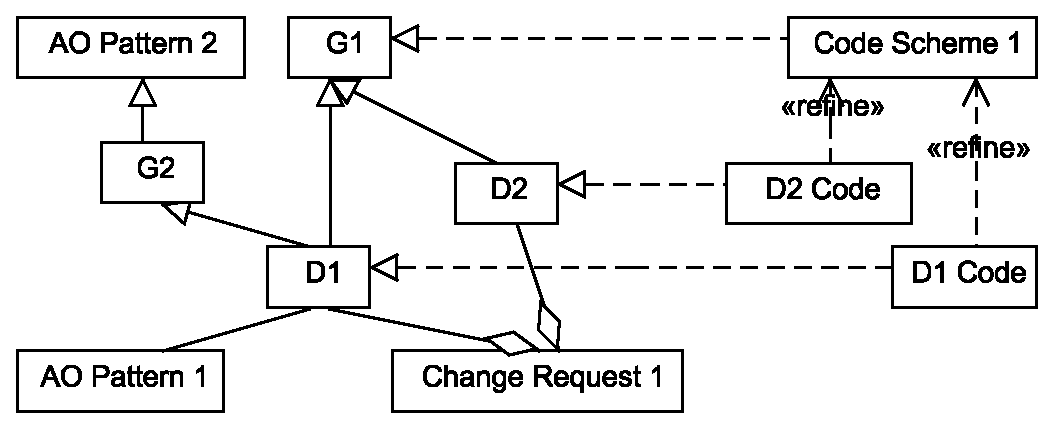
\includegraphics[scale=\magnf]{fig/gen-spec}
% \caption{Generally applicable and domain specific changes.}
% \label{f:gen-spec}
% \end{figure}


% You may include code snippets to explain what you've done:
% \ajset
% \begin{lstlisting}
% public class SMTPServerM extends SMTPServer {
%    . . .
% }
% . . .
% public aspect SMTPServerBackupA {
%    public pointcut SMTPServerConstructor(URL url, String user, String password):
%       call(SMTPServer.new(..)) && args (url, user, password);
%    SMTPServer around(URL url, String user, String password):
%       SMTPServerConstructor(url, user, password) {
%       return getSMTPServerBackup(proceed(url, user, password));
%    }
%    private SMTPServer getSMTPServerBackup(SMTPServer obj) {
%       if (obj.isConnected()) {
%          return obj;
%       }
%       else {
%          return new SMTPServerM(obj.getUrl(), obj.getUser(),
%             obj.getPassword());
%       }
%    }
% }
% \end{lstlisting}

% If you need to display more code, use appendices referring the reader to them, e.g.,
% ``see Appendix~\ref{some} for a more detailed example.''



% \section{Further Steps to\ldots} \label{further}

% You may need several sections to describe your approach.



% \section{Evaluation} \label{eval}

% You may describe your evaluation efforts in a separate, often generically entitled section.

% \subsection{Essential Evaluation} \label{eval-essential}

% Use your own title here.

% \subsection{Threats to Validity} \label{eval-threats}

% \ldots



% \section{Related Work} \label{rw}

% Compare your achievements to related ones achieved by others.



% \section{Conclusions and Further Work} \label{cc}

% % Conclusions
% Emphasize the main results.

% % Further Work
% Indicate what can be done next.

% The concluding section is typically not decomposed into subsections.
% Simply use several paragraphs to present conclusions,
% and then use at least one paragraph to indicate further/future work.


% \bibliographystyle{abbrv} % plain or alpha are fine, too
% \bibliography{bib}

% \appendix
% \section{Some Appendix} \label{some}


% \section{Yet Another Appendix} \label{yetanother}


\end{document}

